\documentclass[xcolor=dvipsnames,10pt]{beamer}
\usepackage{storitemplate}
\usepackage{graphicx}
\usepackage{caption}
\usepackage{subcaption}
\usepackage{algorithm}
\usepackage{algorithmic}

\graphicspath{{./figures/}}

\title[]{The Effect of Recovery Algorithms on Compressive Sensing Background Subtraction.}
\author[]{Rhian Davies, Lyudmila Mihaylova, Nicos Pavlidis, Idris Eckley}
\institute[]{Lancaster University}
\titlegraphic{
\includegraphics[width=2cm,height=0.8cm]{epsrc.pdf}}
 
\date{11th October 2013}

\begin{document}



\begin{frame}[plain]
  \titlepage
\end{frame}

 \begin{frame}{Motivation}
 \begin{figure}[h]
 \centering
 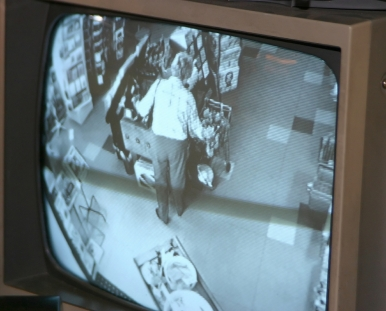
\includegraphics[height=5cm]{cctv}
 \label{fig:cctv}
\end{figure}  
\begin{quote}
\centering  ``Big Brother is Watching You.'' 
 \newline -  George Orwell, 1984  
\end{quote}  

 \end{frame}

		% -- Frame 3-1
\begin{frame}{Background Subtraction}
  \begin{itemize}
  \item Construct, update then subtract. 
\item Not new - many methods exists. 
\item Most traditional methods are not efficient. 
\item CCTV often slowly adaptive background + rare foreground (spatially and temporally)
\item Waste of resources
  \end{itemize}
  \begin{figure}[h]
    \centering
                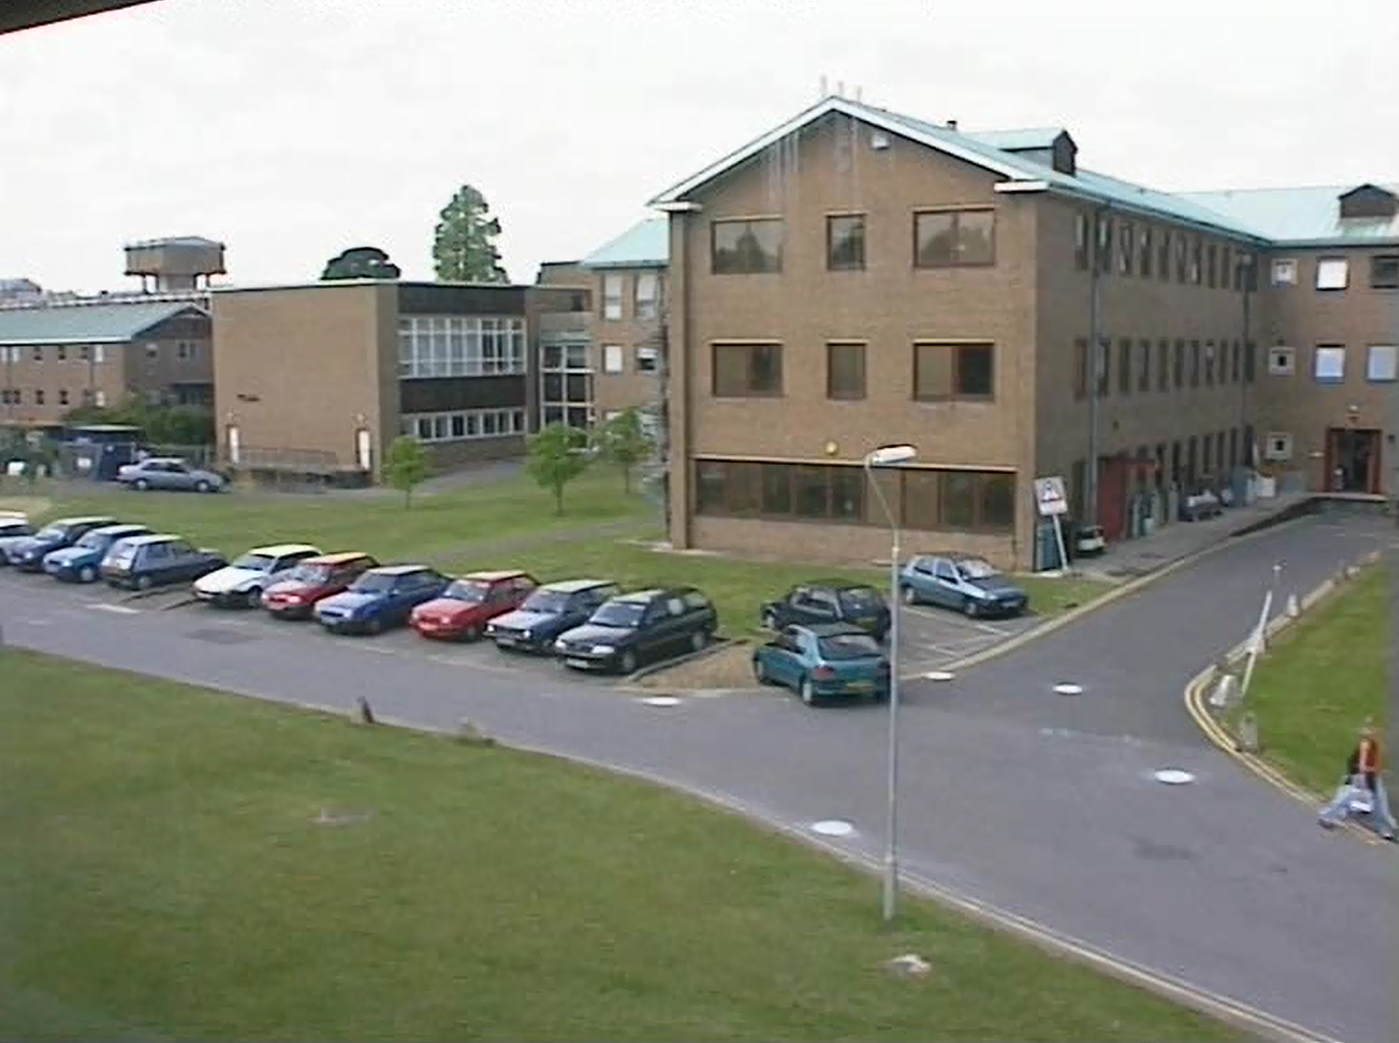
\includegraphics[width=4cm]{camReal}
  \end{figure}

 \end{frame}


 %\begin{frame}
 %  \frametitle{Current Methods}
 %  Surveillance cameras have become ubiquitous in many countries, constantly collecting and storing a huge stream of data. A standard video camera with resolution $720 \times 480$ pixels and a frame rate of 30 frames per second (fps) will need to store  $10,368,000$ pixels for every second of footage collected. Most surveillance cameras are active 24 hours a day which equates to processing over $8.95 \times 10^{11}$ pixels each day for every camera. This large data mass leads to the need for accurate, fast and automated systems to convert raw video into information.

%(These technologies do not exist)
% \end{frame}

 \begin{frame}{What is compressive sensing?}
Compressive sensing is a method of \textbf{reducing the amount of data collected} from a signal without compromising the ability to later \textbf{reconstruct the signal accurately.} This method will only work if the signal of interest is compressible. 

\begin{figure}[h]
        \centering
        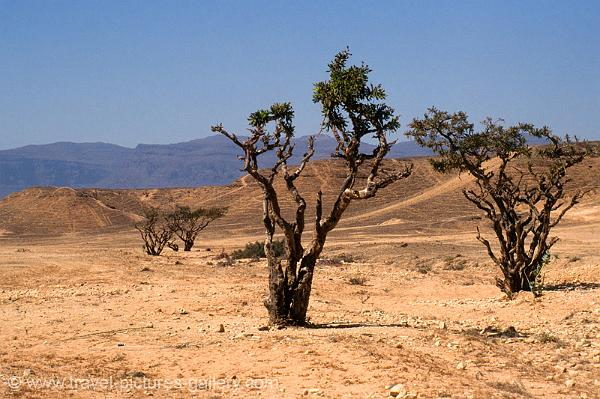
\includegraphics[width = 8cm]{sparseD.jpg}
       \end{figure}

\end{frame}

\begin{frame}
  \frametitle{Sparse and Compressible Signals}
  \begin{itemize}
  \item A signal is known as being \textbf{K-sparse} if $\boldsymbol{x} \in R^N$ can be represented as a linear combination of $K$ basis vectors. 
   \item Interested in $K \ll N$.
     \item If a signal is \textbf{compressible} there exist $K$ large coefficients but the remaining $N-K$ coefficients are only required to be small and not necessarily zero. 
  \end{itemize}
 
  \begin{figure}
    \centering
    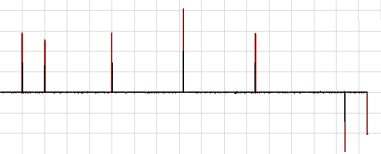
\includegraphics[width = 6cm]{sparse.png}
  \end{figure}

\end{frame}

\begin{frame}
\frametitle{The encoding process.} % Assume that the signal of interest $\pmb{x}$ is of length N.
                 % \begin{itemize}
                 % \item Choose $M$, the number of measurements to take of $\pmb{x}$. $(M < < N).$
                   % \item Create a random measurement matrix $\pmb{\Phi}$ of size $M \times N$. This must satisfy the RIP. 
                   %   \item Calculate measurement $\pmb{y}$ according to equation \eqref{eq:1}.
                  %      \item Reconstruct $\pmb{x}$ using a recovery optimisation method.
                 % \end{itemize}

\begin{figure}[h]
        \centering
        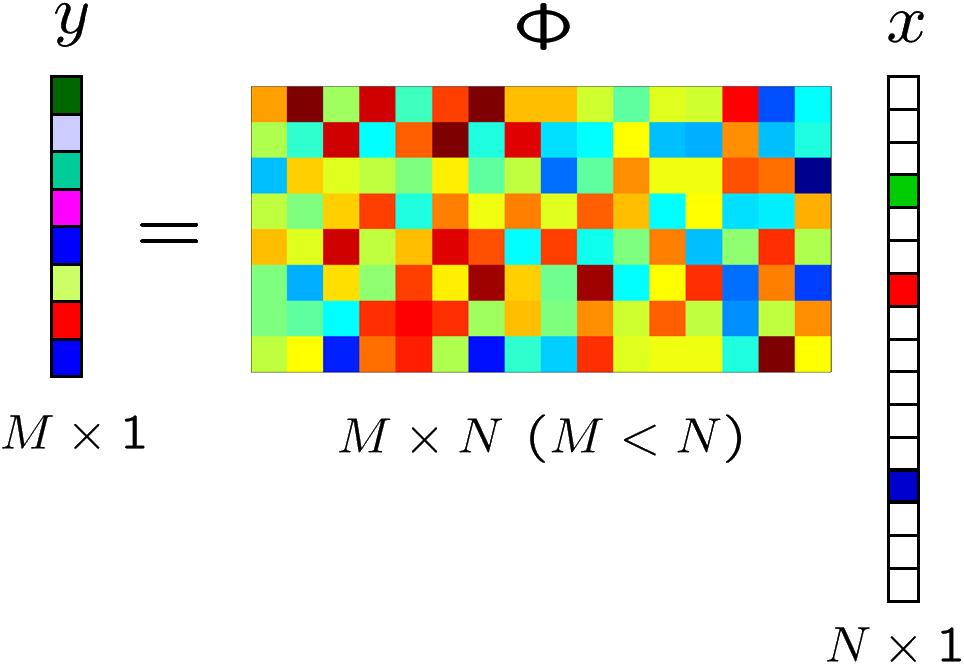
\includegraphics[width = 8cm]{csss}
        \caption{CS measurement process, courtesy of Volkan Cevher.}
      \end{figure}


%\begin{equation}
%  \label{eq:1}
%\pmb{y} =\pmb{\Phi x}
%\end{equation}
%Many vectors $\pmb{\hat{x}}$ can solve equation \eqref{eq:1}, but usually $\pmb{x}$ is the only sparse solution. Therefore if $\pmb{x}$ is known in advance to be sparse, it can in theory be reconstructed exactly from $M$ measurements.
\end{frame}

\begin{frame}{Restricted Isometry Property (RIP)}
 A matrix $\boldsymbol{\Phi}$ satisfies the (RIP) of order $K$ if there exists a $\delta_K  \in (0,1)$ such that 
\begin{equation*}
  \label{eq:40}
  (1 - \delta_k)\|\boldsymbol{x}\|^2_2 \leq\|\boldsymbol{\Phi} \boldsymbol{x}\|^2_2 \leq (1 + \delta_k)\|\boldsymbol{x}\|^2_2,
\end{equation*}

for all $\boldsymbol{x} \in \sum_K = \{\boldsymbol{x}:\|\boldsymbol{x}\|_0 \leq K\} $, \newline

where $\|\boldsymbol{x}\|_0$ is the zero pseudo-norm defined as

\begin{equation*}
\|\boldsymbol{x}\|_0 = \#(i|x_i \neq 0). 
\end{equation*}
 
%WRONG?
%The $l_2$ norm is defined  in equation \eqref{eq:573}. 
%
%\begin{equation}
%\label{eq:573}
%  ||\boldsymbol{x}||_2 = \sum_{i=1}^{N}||\boldsymbol{x_i}^2||
%\end{equation}

If $\boldsymbol{\Phi}$ satisfies the RIP with order $2K$, then $\boldsymbol{\Phi}$ approximately preserves the distance between any pair of $K$-sparse vectors. Unfortunately the task of checking that a matrix satisfies the RIP is a NP-hard problem, but fortunately the RIP will hold true with high probability if $\boldsymbol{\Phi}$ is selected as a random matrix and $M \geq cK\log \frac{N}{K}$, where $c$ is a small constant. 

 % A matrix $\pmb{\Phi}$ satisfies the Restricted Isometry Property (RIP) of order $K$ if there exists a $\delta_K  \in (0,1)$ such that 
%\begin{equation}
%  \label{eq:4}
%  (1 - \delta_k)||\pmb{x}||^2_2 \leq||\pmb{\Phi} \pmb{x}||^2_2 \leq (1 + \delta_k)||\pmb{x}||^2_2,
%\end{equation}
%for all $\pmb{x} \in \sum_K = {\pmb{x}:||\pmb{x}||_0 \leq K} $.
 
%If $\pmb{\Phi}$ satisfies the RIP with order $2K$, then $\pmb{\Phi}$ preserves the distance between any pair of $K$-sparse vectors, making the recovery procedure possible.
\end{frame}

      \begin{frame}{Recovery of sparse transforms}
        \begin{itemize}
\item Solve $\boldsymbol{y} = \boldsymbol{\Phi x}$ , infinitely many solutions! Fat $\boldsymbol{\Phi}$ implies underdetermined system. 
\item We know that $\boldsymbol{x}$ was \textbf{sparse} 
       %   \item $\Delta(y, \Phi) = x$
%\item Ideally use the $\ell_0$ norm. 
\item What algorithms can we use to decode? 
\item Convex Optimisation or Greedy Algorithms or something else...?
        \end{itemize}
\end{frame}

\begin{frame}
  \frametitle{Using $\ell_1$ minimization to promote sparsity}
%\begin{equation*}
%  \label{eq:3}
%  \hat{x} = \text{arg} min_{y = \phi x} ||x||_0 \newline
%\mbox{where}\vspace{1cm} \|\boldsymbol{x}\|_0 = \#(i|x_i \neq 0).  
%\end{equation*}

\begin{equation*}
\label{eq:57}
  \|\boldsymbol{x}\|_1 = \sum_{i=1}^{N}|x_i|
\end{equation*}

Originally used in geophysics to aid detection of sparse spike trends in earthquake data, optimisation based on the $l_1$ norm can closely approximate compressible signals with high probability.  
\begin{equation*}
  \label{eq:4}
  \min_{\boldsymbol{x}} ||\boldsymbol{x}||_1 \text{ subject to } \boldsymbol{y} = \boldsymbol{\Phi} \boldsymbol{x}.
\end{equation*}


\end{frame}

\begin{frame}{Orthogonal Matching Pursuit}
\begin{algorithm}[H]
\caption{Orthogonal Matching Pursuit}  
\begin{algorithmic}
\STATE{Define the columns of $\boldsymbol{\Phi}$ to be $\varphi_1, \varphi_2, \hdots, \varphi_N$.}% each of length $M$.}
\REQUIRE $\boldsymbol{r_0} = \boldsymbol{y}, \Lambda_0 = \emptyset$ and iteration counter $i = 1$
\FOR{$i < T$} % \COMMENT{T is the maximum iteration count.}
 \STATE  $\lambda_t = \text{argmax }_{j=1,\hdots,N}|<r_{t-1}, \varphi_j>|$ \\  \COMMENT{Find the index for the column of $\Phi$ with the greatest contribution.}
 \STATE  $\Lambda_t = \Lambda_{t-1} \cup {\lambda_t}$, $\Phi_t = [\boldsymbol{\Phi_{t-1}}, \varphi_{\lambda_t}]$ \\ \COMMENT{Keeps track of the columns used.}
\STATE   $\boldsymbol{x_t} = \text{argmin}_{\boldsymbol{x}} || \boldsymbol{y} - \boldsymbol{\Phi_t} \boldsymbol{x}||_2$  \\ \COMMENT{Updates the signal estimate.}
\STATE  $\boldsymbol{r_t} =  \boldsymbol{y} - \boldsymbol{\Phi_t} \boldsymbol{x_t}$ \\ \COMMENT {Updates the measurement residual.}
\ENDFOR
\RETURN  $\boldsymbol{\hat{x}}$
\end{algorithmic}
\end{algorithm}

% We shall define the columns of $\Phi$ to be $\varphi_1, \varphi_2, \hdots, \varphi_N$ each of length $M$. 

%\begin{itemize}
%\item Inputs: Measurement matrix $\Phi$ and observations $y$.
%\item Initialize: $r_0 = y, \Lambda_0 = \emptyset$
%\item for $t=1, t:=t+1$ until stopping criterion is met \emph{do}
%\item Step 1: Find the index for the column of $\Phi$ which satisfies $\lambda_t = \text{argmax }_{j=1,\hdots,N}|<r_{t-1}, \varphi_j>|$ 
%\item Step 2: Keeps track of the columns used. $\Lambda_t = \Lambda_{t-1} \cup {\lambda_t}$, $\Phi_t = [\Phi_{t-1}, \psi_{\lambda_t}]$ 
%\item Step 3: Update the estimate of the signal.  $x_t = \text{argmin}_x || v - \Phi_tx||_2$ .
%\item Step 4: Update the measurement residual. $r_t =  y - \Phi_t x_t$.  
%\item Output: Estimated sparse vector $\hat{x}$
%\end{itemize}
\end{frame}

\begin{frame}
  \frametitle{Recap}
  \begin{figure}[h]
    \centering
    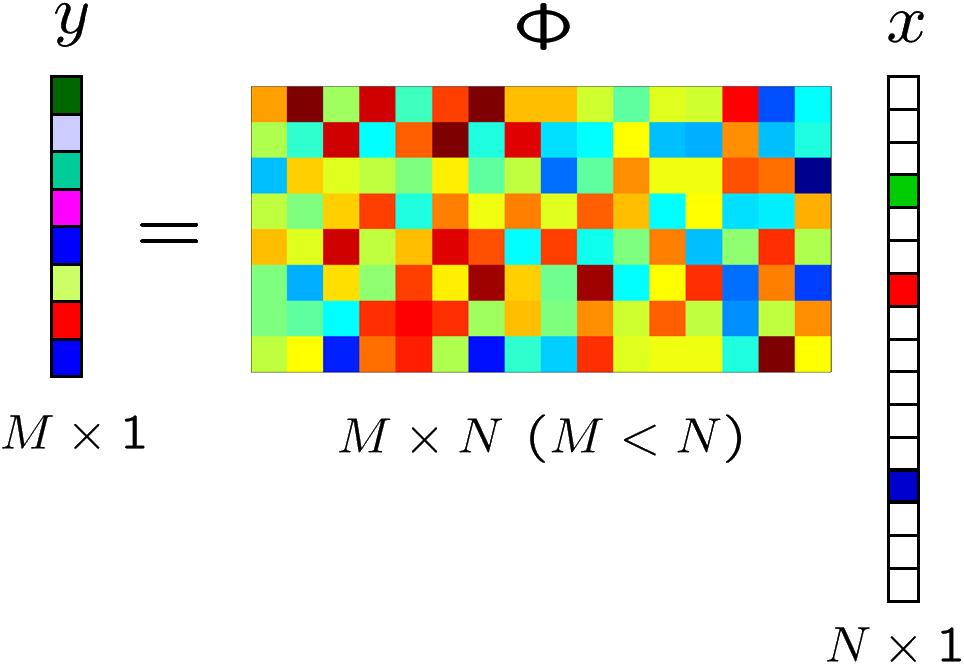
\includegraphics[width = 8cm]{csss}
  \end{figure}
\end{frame}
               
  \begin{frame}{Sparsity}    

\begin{figure}
        \centering
        \begin{subfigure}[b]{0.4\textwidth}
                \centering
                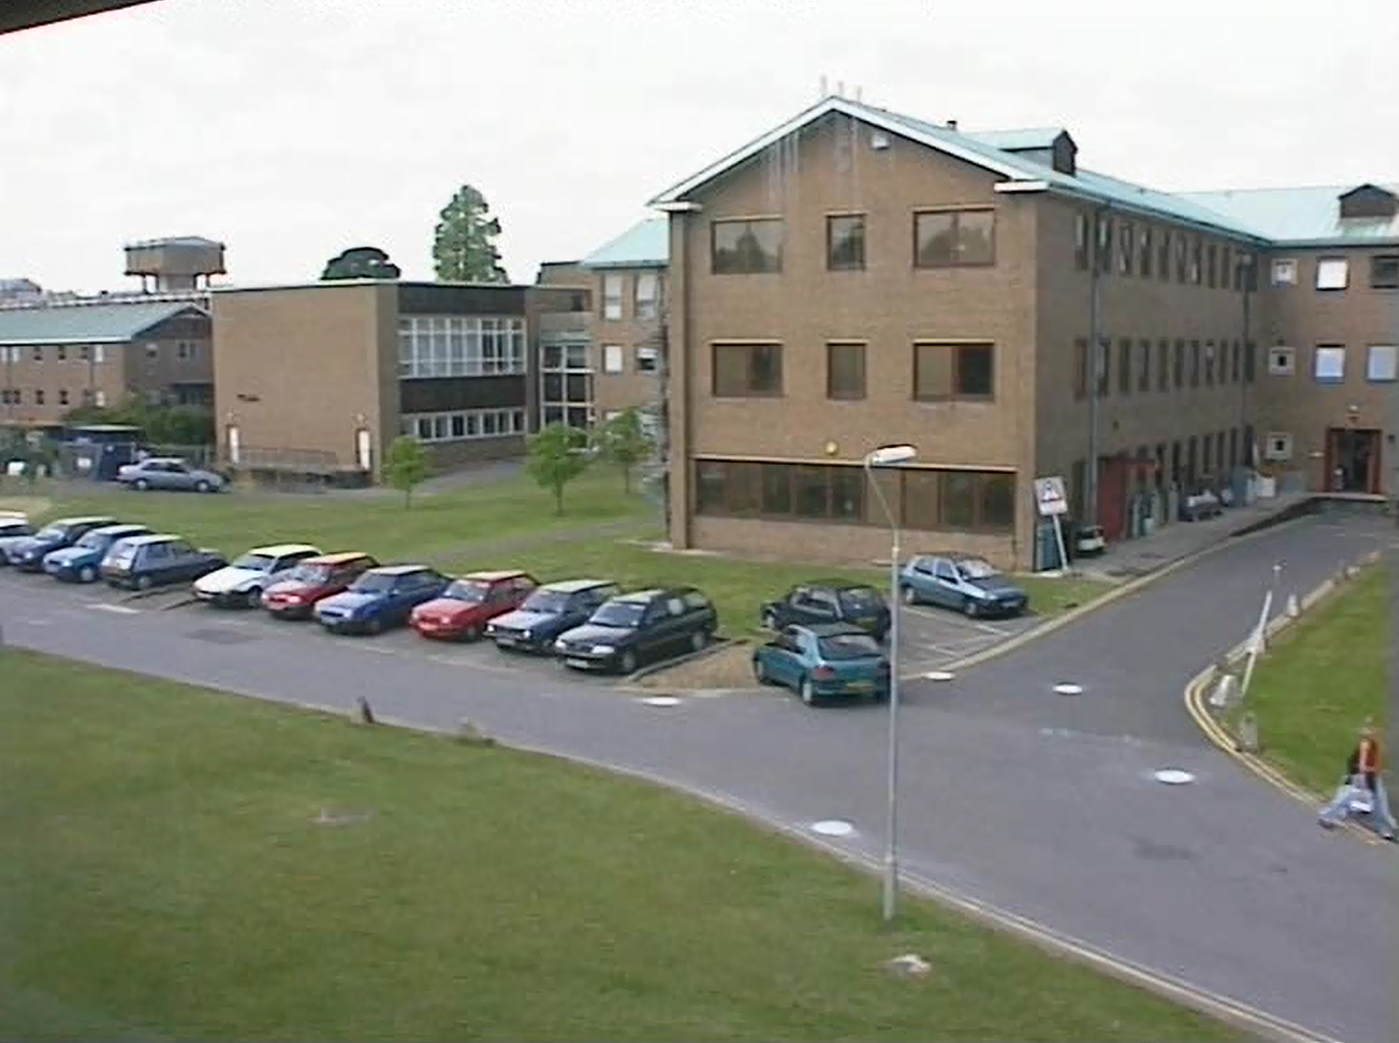
\includegraphics[width=\textwidth]{camReal}
                \caption{Test frame}
               % \label{fig:gull}
        \end{subfigure}%
        ~ %add desired spacing between images, e. g. ~, \quad, \qquad etc.
          %(or a blank line to force the subfigure onto a new line)
        \begin{subfigure}[b]{0.4\textwidth}
                \centering
                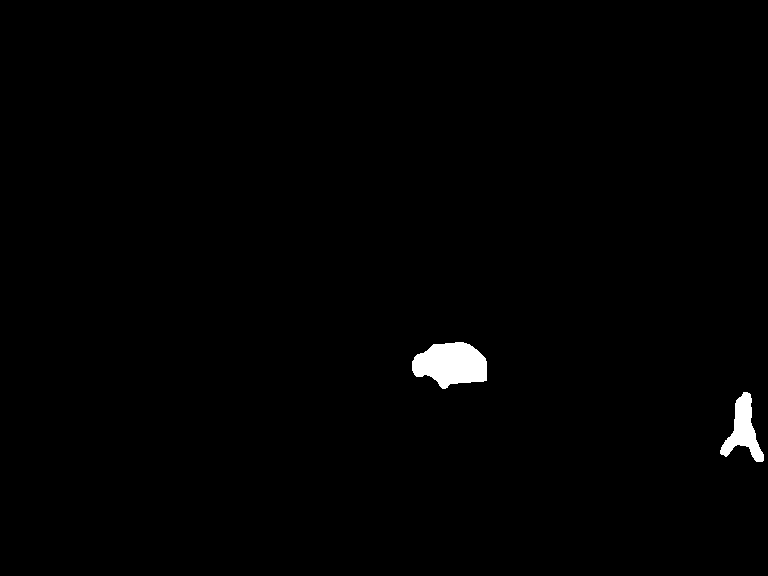
\includegraphics[width=\textwidth]{camGT}
                \caption{Ground truth}
              %  \label{fig:tiger}
        \end{subfigure}
\caption{The spatial sparsity of foreground. A frame from the PETS data set and the corresponding foreground in white. In this example, less than 1\% of the frame is foreground, as N=442,368 and K=3862.  }\label{fig:sparse}
\end{figure}

 \end{frame}

 \begin{frame}
   \frametitle{Encoding}
   \begin{figure}[h]
     \centering
     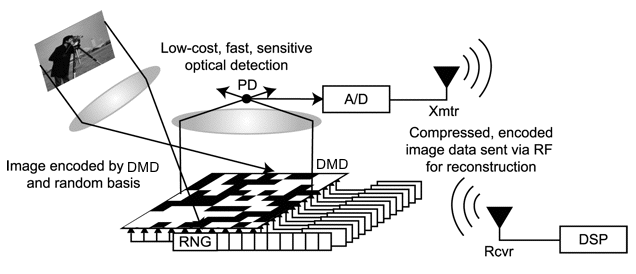
\includegraphics[width = 10cm]{spc}
     \caption{The single pixel camera}
   \end{figure}
    \end{frame}

      
% \begin{frame}
%   \frametitle{Compressive Sensing Background Subtraction}
%   IMAGE
% \end{frame}

      % -- Frame 3-34 
      \begin{frame}{Compressive Sensing Background Subtraction.}

\begin{algorithm}[H]
%\caption{Orthogonal Matching Pursuit}  
\begin{algorithmic}
\REQUIRE Initial compressed background $y^b_0$
\FOR{all t} % \COMMENT{T is the maximum iteration count.}
\STATE Compressively Sense (Encode) $y_t = \Phi x_t$.
\STATE Reconstruct (Decode)   $\hat{x_t} = \Delta (y_t - y^b_t)$
\STATE Update Background  $y^b_{t+1} = \alpha y_{t+1} + (1 - \alpha)y^b_t$
\RETURN  $\boldsymbol{\hat{x_t}}$
\ENDFOR

\end{algorithmic}
\end{algorithm}
\end{frame}

\begin{frame}
  \frametitle{Results}

   \begin{table}[ht!]
%\caption{CS$_{\ell_1}$ and CS$_{\text{OMP}}$ segmentation for 3 test scenes ($N = 4096, M = 2048, \alpha = 0.05$). }
\centering
\begin{tabular}{cccc}
\parbox[top]{20mm}{Original} &  \parbox[top]{20mm}{Ground Truth} & \parbox[top]{20mm}{CS$_{\ell_1}$} & \parbox[top]{20mm}{CS$_{\text{OMP}}$} \\
 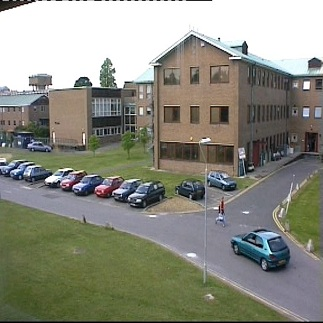
\includegraphics[width=16mm]{1}& 
\includegraphics[width=16mm]{GTB} & 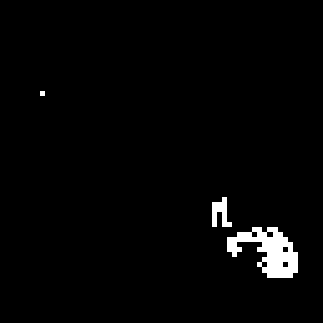
\includegraphics[width=16mm]{1l} & 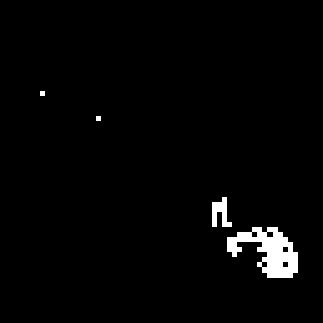
\includegraphics[width=16mm]{1o} \\
 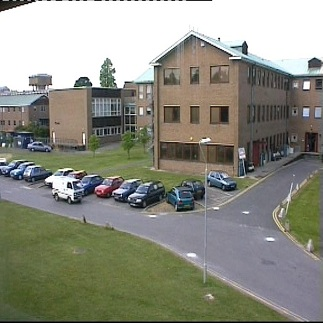
\includegraphics[width=16mm]{2}& 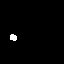
\includegraphics[width=16mm]{GTD} & 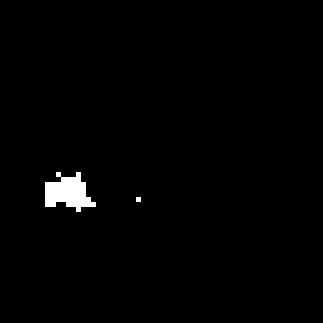
\includegraphics[width=16mm]{2l} & 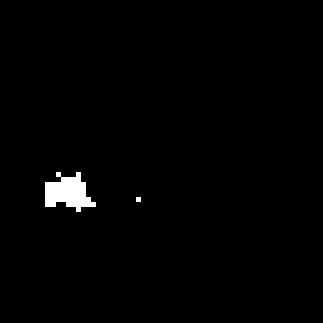
\includegraphics[width=16mm]{2o} \\
 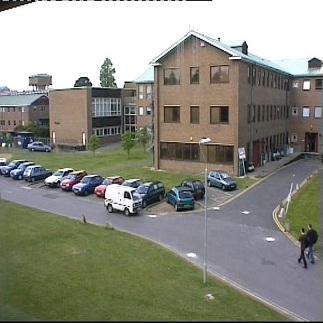
\includegraphics[width=16mm]{3}& 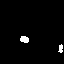
\includegraphics[width=16mm]{GTE} & 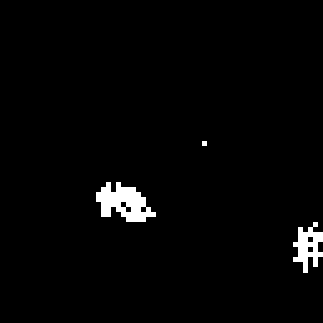
\includegraphics[width=16mm]{3l} & 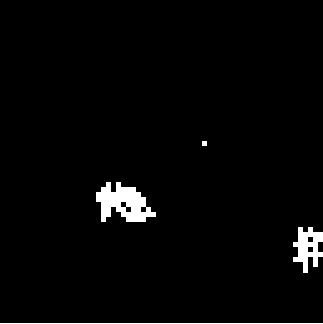
\includegraphics[width=16mm]{3o} \\
 \end{tabular}
\label{tab:gt}
\end{table}

\end{frame}

\begin{frame}
  \frametitle{Results}
  \begin{figure}[t]
  \centering
  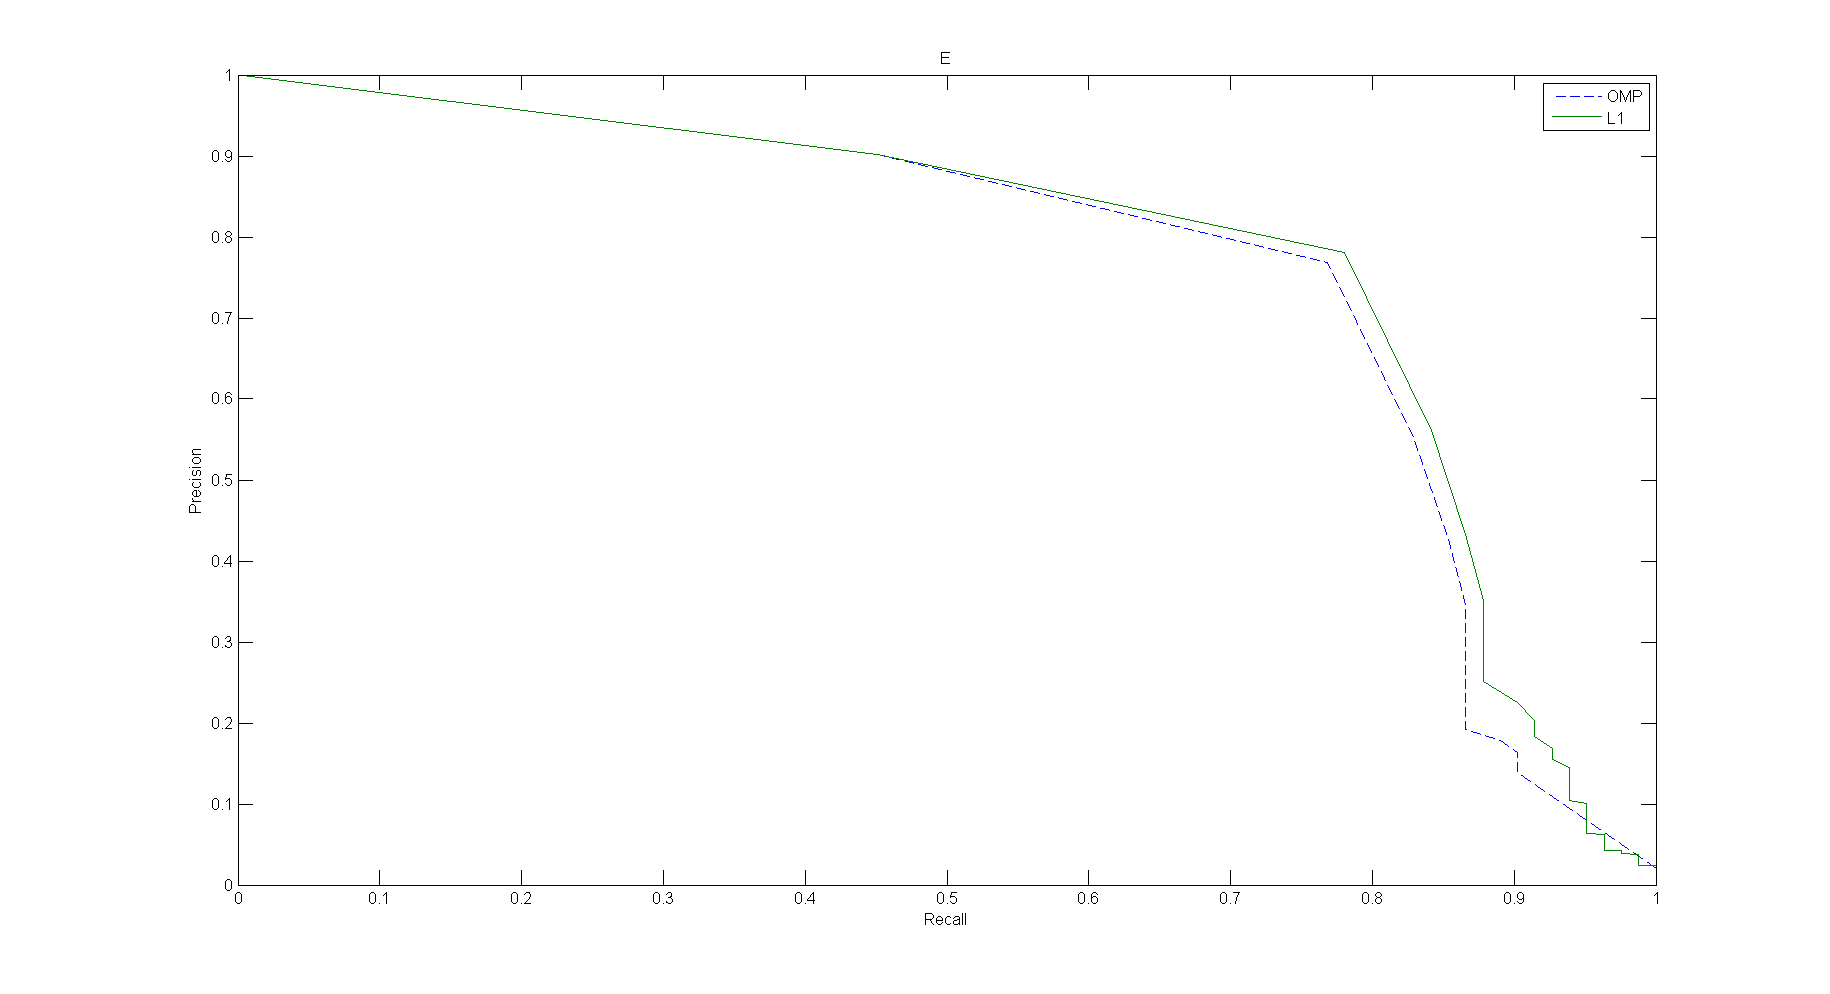
\includegraphics[width = 10cm]{Epr}
  \caption{Precision-Recall Curves for the 3rd test frame}
  \label{fig:precrec}
\end{figure}
\end{frame}
      
\begin{frame}
  \frametitle{Results}
  
\begin{figure}[t]
  \centering
  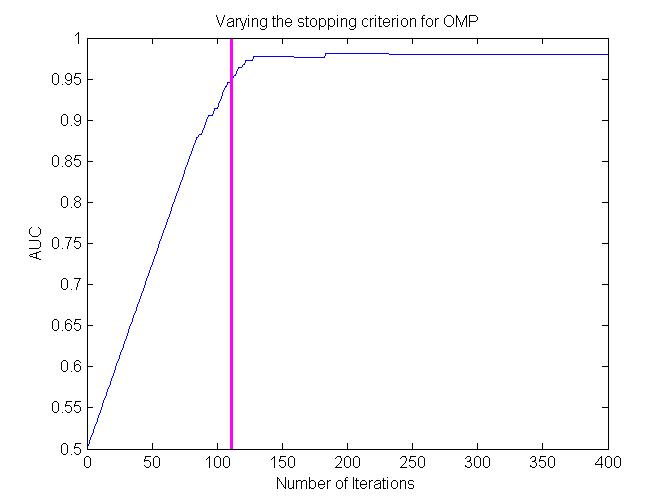
\includegraphics[width = 7cm]{varyingSComp}
  \caption{Selection of the stopping criterion for OMP}
  \label{fig:omp}
\end{figure}
\end{frame}

\begin{frame}
  \frametitle{Results}
  \begin{figure}[t]
  \centering
  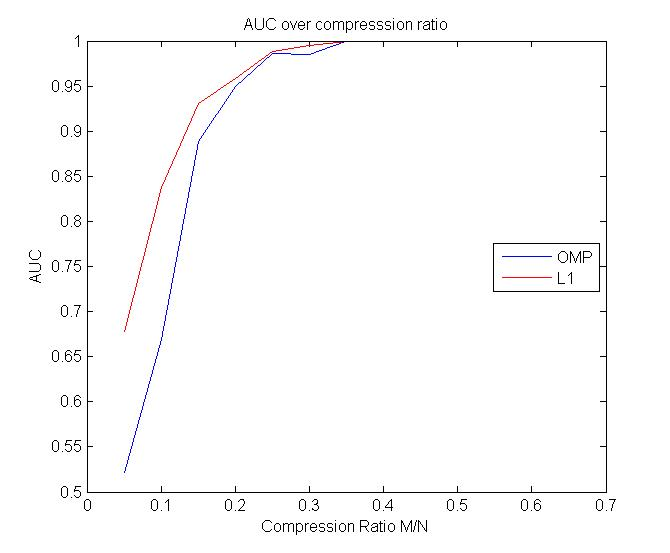
\includegraphics[width = 7cm]{AUCcompressionRatio}
  \caption{AUC over Sparsity Ratio}
  \label{fig:sr}
\end{figure}
\end{frame}



\begin{frame}
  \frametitle{Conclusion and thoughts for the future.}
  \begin{itemize}
  \item $\ell_1$ minimisation outperforms OMP, but it's close!
\item Effect of the stopping criterion is vital for OMP - adaptive methods needed?
\item Ideal boundaries for compression ratio of $\frac{M}{N}$ around $25 \% - 35 \%$ 
\item Can we incorporate prior information to aid the recovery process?
  \end{itemize}
\end{frame}
      \begin{frame}
        \frametitle{Thanks! }

\Large{
Rhian Davies
\newline
\newline
r.davies3@lancs.ac.uk
\newline
\url{www.lancs.ac.uk/~daviesr3} } 
       \end{frame}

\begin{frame}
  \frametitle{Precision and Recall Definitions}
  Recall is defined as the fraction of correctly identified foreground pixels over the number of ground truth foreground pixels which can be written mathematically as
\begin{equation}
  \label{eq:1}
\text{Recall} = \frac{TP}{TP + FN}. 
\end{equation}
Precision is defined to be the fraction of correctly identified foreground pixels over the number of detected foreground pixels in total, or when written mathematically
\begin{equation}
  \label{eq:2}
\text{Precision} = \frac{TP}{TP + FP}.
\end{equation} 

\end{frame}

 \end{document}

 \begin{frame}
   \frametitle{Making every pixel count.}
 \begin{figure}
        \centering
        \begin{subfigure}[b]{0.45\textwidth}
                \centering
                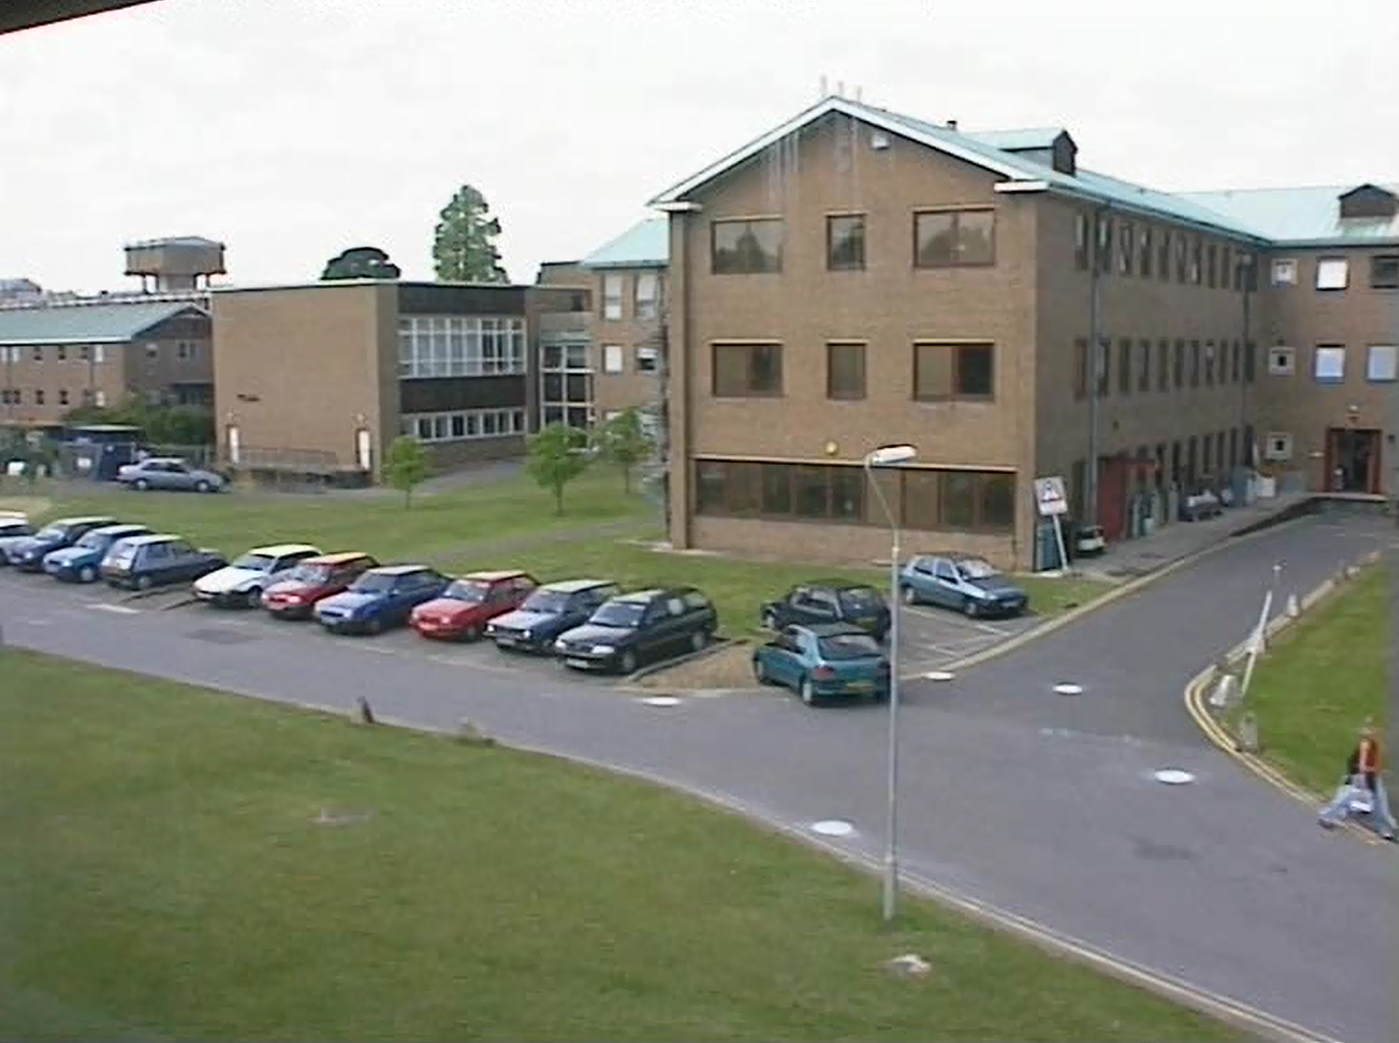
\includegraphics[width=\textwidth]{camReal}
                \caption{C.S.I ``magic''}
              \end{subfigure}%
        ~ %add desired spacing between images, e. g. ~, \quad, \qquad etc.
          %(or a blank line to force the subfigure onto a new line)
        \begin{subfigure}[b]{0.45\textwidth}
                \centering
                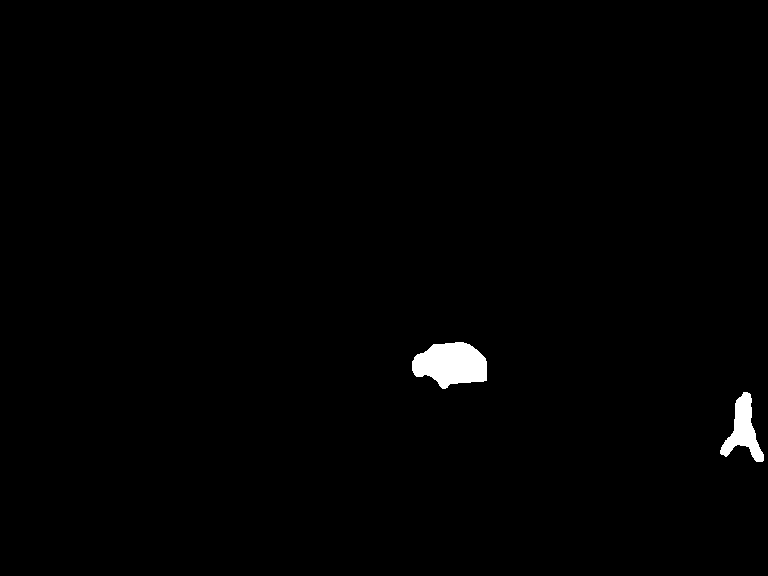
\includegraphics[width=\textwidth]{camGT}
                \caption{The single pixel camera. }
              %  \label{fig:tiger}
        \end{subfigure}
\end{figure}

 Acquire information in a compressed manner, then reconstruct.

 \end{frame}

